\documentclass{article}
%%%%%%%%%%%%
% PACKAGES %
%%%%%%%%%%%%
\usepackage[utf8]{inputenc}
\usepackage{lastpage}

\usepackage{todonotes}

\usepackage[urldate=long]{biblatex}
\addbibresource{sections/references.bib}
\usepackage[hidelinks]{hyperref}

% Changes the paragraph indentations to newlines
\usepackage[parfill]{parskip}

\usepackage[a4paper]{geometry}

\usepackage{minted}
% \usemintedstyle{vs}
\newenvironment{haskell}{\VerbatimEnvironment\begin{center}\begin{minted}[escapeinside=!!]{haskell}}{\end{minted}\end{center}}

\newcommand{\inlinehaskell}[1]{\mintinline[escapeinside=!!]{haskell}{#1}}

\usepackage{float}

\usepackage{graphicx}
\graphicspath{ {images} }

\usepackage{fancyhdr}
\pagestyle{fancy}
\fancyhf{} % Clears the default header and footers
\fancyhead[L]{Jort van Gorkum — Master's Thesis}
\fancyhead[R]{Page \thepage\ of \pageref{LastPage}}

\linespread{1.3}

\usepackage[inline]{enumitem}

\usepackage{multirow}

%%%%%%%%%%%%
% DOCUMENT %
%%%%%%%%%%%%
\begin{document}

\begin{titlepage}
    \fontsize{12pt}{15pt}\selectfont
    \begin{center}
      \vspace*{4cm}
  
      Master's Thesis
  
      \vspace{0.5cm}
  
      {
        \fontsize{20.74pt}{20.74pt}\selectfont
        \parbox[]{13cm} {
          \centering
          Incremental Cata Computation \\ for Generic Data Types
        }
      }
        
      \vspace{1.25cm}
      
      Jort van Gorkum - 6142834 \\
      Computing Science - Programming Technology \\
      Utrecht University \\
      
      \vspace{1.25cm}
      
      Supervisors: \\
      Dr. Wouter Swierstra, Dr. Trevor McDonell \\
      
      \vspace{1cm}
  
      \today
    \end{center}
  \end{titlepage}

% \chapter{Introduction}

\todo[inline]{Write more context}
\todo[inline]{Add a problem statement}

\todo[inline]{Add why my thesis is unique}

Incremental computation is an approach to improve performance by computing only the result of the changed parts of the input, instead of computing the entire result. To determine what parts of the input has changed, we provide a \textit{Zipper} which can be used by the user to efficiently update the previous input to a new input and keeps track of the changes to the input. As a result, we know which parts of the input stays the same. Therefore, we can reuse the results of a previously performed computation for the same input\footnote{The technique for reusing results based on input is called \textit{memoization}}.   

The task of implementing incremental computation for Haskell is explained in Chapter \ref*{chap-spec-impl}. However, the task for implementing incremental computation for multiple datatypes, becomes repetitive and error-prone. To prevent writing implementations for every datatype, we use datatype-generic programming. Datatype-generic programming is a technique that uses the structure of a datatype to define functions for a large class of datatypes, which is explained in more detail in Chapter \ref*{chap-dat-gen-program}. Then, using the Haskell generics library \texttt{regular}, we implement the generic version. In Chapter \ref*{chap-gen-impl}, the generic implementation is explained and additionally describe: complexity, different garbage collection strategies and different data structures for storing results. 

To illustrate how the incremental computation functionality is used, an example is presented which implements the \textbf{max-path-sum} in a non-incremental and an incremental manner. The max-path-sum function traverses through a tree and returns the sum of the path with the highest value. For the example, we first define the definition of a tree and an example tree which is used as input for the max-path-sum. Then, the non-incremental function (\inlinehaskell{maxPathSum}) is implemented, by returning the value for the leaf; and for the node recursively calling the children and determine the highest value between the children and adding it to its own value.

\begin{minted}{haskell}
data BinTree = Leaf Int
             | Node BinTree Int BinTree 
             
exampleTree :: BinTree    
exampleTree = Node (Node (Leaf 8) 7 (Leaf 1)) 3 (Node (Leaf 5) 4 (Leaf 2))

-- The non-incremental implementation of max-path-sum
maxPathSum :: BinTree -> Int
maxPathSum (Leaf x)     = x
maxPathSum (Node l x r) = x + max (maxPathSum l) (maxPathSum r)

> maxPathSum exampleTree
    18

> let exampleTree' = update (const (Leaf 6)) [Bttm] exampleTree

> maxPathSum exampleTree'
    16
\end{minted}

The incremental implementation, first adds hashes to the input which represent the internal data structure to the data structure (also known as a \textit{merkle tree}). This is used to efficiently check what parts of the input has changed. Then, the initial computation is performed which gives the result and a map of all the intermediate results. Next, the tree gets updated, in this case the bottom left leaf (\inlinehaskell{Leaf 8}) is replaced with \inlinehaskell{Leaf 6}. Finally, the updated tree is recomputed reusing the previously computed results. As a result, the complete right side of the root node did not have to be recomputed, because it stayed the same.

\todo[inline]{Add the explanation of that we use the Zipper for updating the Tree}

\begin{minted}{haskell}
-- The incremental implementation of max-path-sum
incMaxPathSum :: BinTree -> Int
incMaxPathSum (Leaf_ x)     = x
incMaxPathSum (Node_ l x r) = x + max l r

-- Add hashes to data structure
> let merkleTree = merkle exampleTree

-- Initial computation
> let (y, m) = cataMerkle incMaxPathSum (merkleTree)
    (18, { "6dd": 18, "5df": 15, "fa0": 8, "8d0": 1, "f3b": 9, "84b": 5
         , "1ad": 2 })

-- Update Tree
> let merkleTree' = update (const (merkle (Leaf 6))) [Bttm] merkleTree

-- Incremental computation
> cataMerkleMap incMaxPathSum m (merkleTree')
    (16, { "6dd": 18, "5df": 15, "fa0": 8, "bbd": 16, "91c": 13, "3af": 6
         , "8d0": 1, "f3b": 9, "84b": 5, "1ad": 2 })
\end{minted}

\section{Contributions}

The main contributions of the Thesis are the following:

\begin{itemize}
    \item We define an algorithm for incremental computation over recursive data structures. The algorithm uses hashes for comparing if the data structures are equal in a constant time and a Zipper to efficiently update the recursive data structure without rehashing the entire data structure.
    \item We use datatype-generic programming to write a generic version of the algorithm, to support a large class of datatypes, namely \textit{regular datatypes}.
    \item We use pattern synonyms, to make the developer experience the same as implementing a non-incremental algorithm.
    \item We define cache addition policies and cache replacement policies to optimize the performance/memory usage for different use-cases.
\end{itemize}


% \newpage
% \section{Background}

\subsection{Generic programming in Haskell}
\todo[inline]{Introduce generic programming and how it works}

\subsubsection{Pattern Functors vs Sums of products}
\todo[inline]{Describe the differences between defining generic data types}

\subsubsection{Mutually recursive datatypes}
\todo[inline]{Describe what mutually recursive datatypes are and why do we need to know about it}

\section{Zipper}

% \question{Add a visual example?}

The Zipper is a technique of representing a data structure by keeping track of how the data structure is being traversed through. The Zipper was first described by \citeauthor{huet1997zipper}\cite{huet1997zipper} and is a solution for efficiently updating pure recursive data structures in a purely functional programming language (e.g., Haskell). This is accomplished by keeping track of the downward current subtree and the upward path, also known as the \textit{location}. 

To keep track of the upward path, we need to store the path we traverse to the current subtree. The traversed path is stored in the \texttt{Cxt} datatype. The \texttt{Cxt} datatype represents three options the path could be at: the \texttt{Top}, the path has traversed to the left (\texttt{L}), or the path has traversed to the right (\texttt{R}).

\begin{minted}{haskell}
data Cxt a = Top
           | L (Cxt a) (Tree a) a
           | R (Cxt a) (Tree a) a

type Loc a = (Tree a, Cxt a)

enter :: Tree a -> Loc a
enter t = (t, Top)           
\end{minted}

Using the \texttt{Loc}, we can define multiple functions on how to traverse through the \texttt{Tree}. Then, when we get to the desired location in the \texttt{Tree}, we can call the \texttt{modify} function to change the \texttt{Tree} at the current location.

\begin{minted}{haskell}
left :: Loc a -> Loc a
left (Node l x r, c) = (l, L c r x)

right :: Loc a -> Loc a
right (Node l x r, c) = (r, R c l x)

up :: Loc a -> Loc a
up (t, L c r x) = (Node t x r, c)
up (t, R c l x) = (Node l x t, c)

modify :: (Tree a -> Tree a) -> Loc a -> Loc a
modify f (t, c) = (f t, c)
\end{minted}

Eventually, when every value in the \texttt{Tree} has been changed, the entire \texttt{Tree} can then be rebuilt using the \texttt{Cxt}. By recursively calling the \texttt{up} function until the top is reached, the current subtree gets rebuilt. And when the top is reached, the entire tree is then returned.

\begin{minted}{haskell}
leave :: Loc a -> Loc a
leave l@(t, Top) = l
leave l = top (up l)
\end{minted}

\subsection{Zipper \texttt{TreeH}}

The implementation of the Zipper for the \texttt{TreeH} datatype is the same as for the \texttt{Tree} datatype. However, the \texttt{TreeH} also contains the hash of the current and underlying data structure. Therefore, when a value is modified in the \texttt{TreeH}, all the parent nodes of the modified value needs to be updated. 

The \texttt{updateLoc} function modifies the value at the current location, then checks if the location has any parents. If the location has any parents, go up to that parent, update the hash of that parent and recursively update the parents hashes until we are at the top of the data structure. Otherwise, return the modified locations, because all the other hashes are not affected by the change. 

\begin{minted}{haskell}
updateLoc :: (TreeH a -> TreeH a) -> Loc a -> Loc a
updateLoc f l = if top l' then l' else updateParents (up l')
    where
        l' = modify f l

        updateParents :: Loc a -> Loc a
        updateParents (Loc x Top) = Loc (updateHash x) Top
        updateParents (Loc x cs)  = updateParents $ up (Loc (updateHash x) cs)
\end{minted}

Then, the \texttt{update} function can be defined using the \texttt{updateLoc} function, by first traversing through the data structure with the given directions. Then modifying the location using the \texttt{updateLoc} function and then leave the location and the function results in the updated data structure.

\begin{minted}{haskell}
update :: (TreeH a -> TreeH a) -> [Loc a -> Loc a] -> TreeH a -> TreeH a 
update f dirs t = leave $ updateLoc f l'
    where
        l' = applyDirs dirs (enter t)
\end{minted}

\subsection{Comparison of Generic programming libraries in Haskell}
\todo[inline]{Describe the differences between Generic programming libraries in Haskell}

\subsubsection{Regular}
\todo[inline]{Describe the workings of Regular with an example}

\begin{minted}{haskell}
data Tree a = Leaf a
            | Node (Tree a) a (Tree a)

$(deriveAll ''Tree "PFTree")
type instance PF (Tree a) = PFTree a
\end{minted}

\begin{minted}[escapeinside=!!]{haskell}
t :: Tree Int
t = Node (Leaf 1) 2 (Leaf 3)

pt :: Fix (PF (Tree a)) !$\equiv$! Fix (C (K a) :+: C (I :*: K a :*: I))
pt = In (from t)
\end{minted}

\begin{minted}{haskell}
cata :: Functor f => (f a -> a) -> Fix f -> a
cata alg t = alg (fmap (cata alg) (out t))

cataSum :: Fix (PF (Tree Int)) -> Int
cataSum = cata f
  where
    f :: PF (Tree Int) Int -> Int
    f (L (C (K x)))               = x
    f (R (C (I l :*: K x :*: r))) = l + x + r
\end{minted}

% Zipper
\begin{minted}{haskell}
data Loc :: * -> * where
  Loc :: (Regular a, Zipper (PF a)) => a -> [Ctx (PF a) a] -> Loc a

data family Ctx (f :: * -> *) :: * -> * 

class Functor f => Zipper f where
  cmap        :: (a -> b) -> Ctx f a -> Ctx f b
  fill        :: Ctx f a -> a -> f a
  first, last :: f a -> Maybe (a, Ctx f a)
  next, prev  :: Ctx f a -> a -> Maybe (a, Ctx f a)
\end{minted}

\begin{minted}{haskell}
-- Move down to the leftmost child. Returns 'Nothing' if the
-- current focus is a leaf.
down :: Loc a -> Maybe (Loc a)
down (Loc x cs) = first (from x) >>= \(a,c) -> return (Loc a (c:cs))
\end{minted}

\subsection{HDiff}
\todo[inline]{Write a piece about what HDiff does and how it suggests the use of Merkle trees}
\todo[inline]{Write a piece about the suggestion of storing the hashes inside a Trie datastructure}

\subsection{Selective Memoization}
\todo[inline]{Write a piece about what to look out for with memoization}




\newpage
\chapter{Experiments}

\section{Execution Time}
% \begin{figure}[H]
%     \centering
%     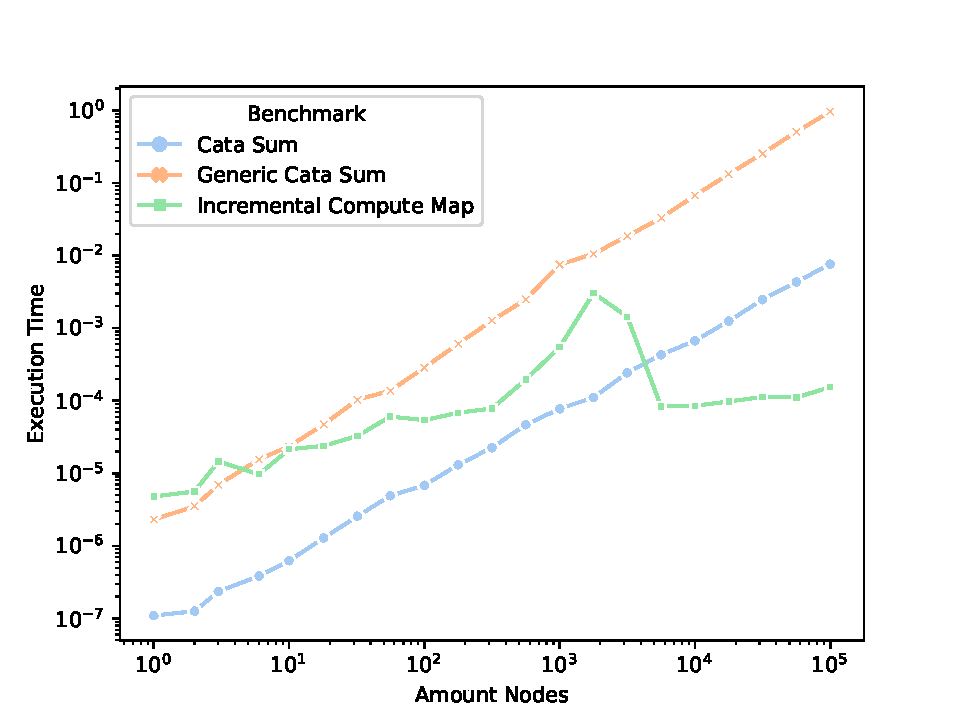
\includegraphics[width=.6\textwidth]{plots/run-2/time/all_benchmarks.pdf}
%     \caption{Overview execution time}
%     \label{fig-exec-time-overview}
% \end{figure}

% \begin{figure}[H]
%     \centering
%     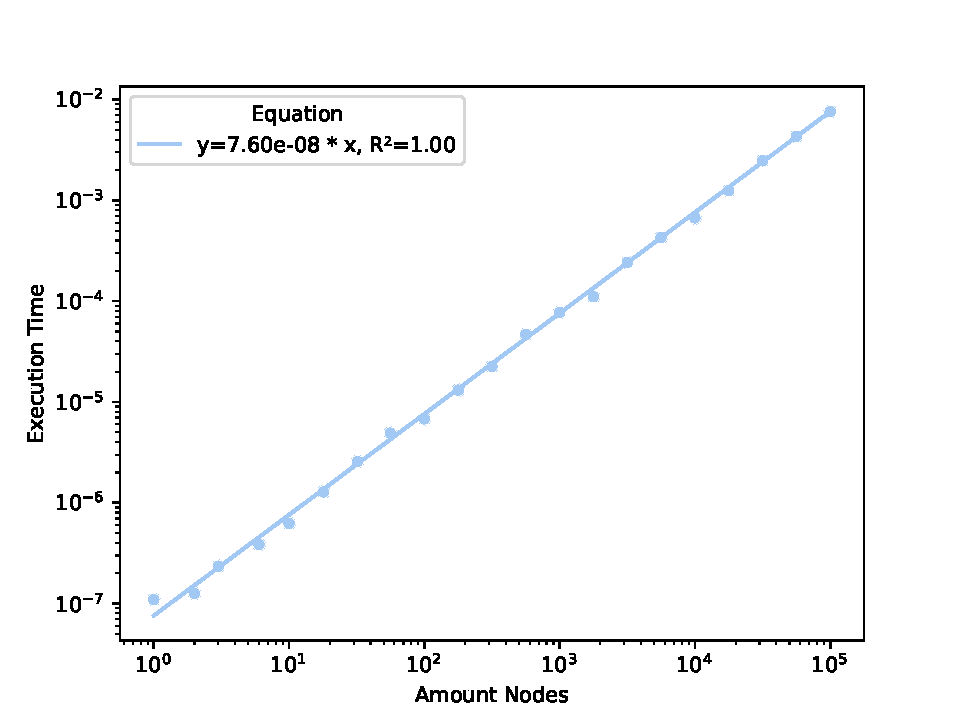
\includegraphics[width=.6\textwidth]{plots/run-2/time/benchmark_cata_sum.pdf}
%     \caption{Execution time for Cata Sum}
%     \label{fig-exec-time-cata-sum}
% \end{figure}

% \begin{figure}[H]
%     \centering
%     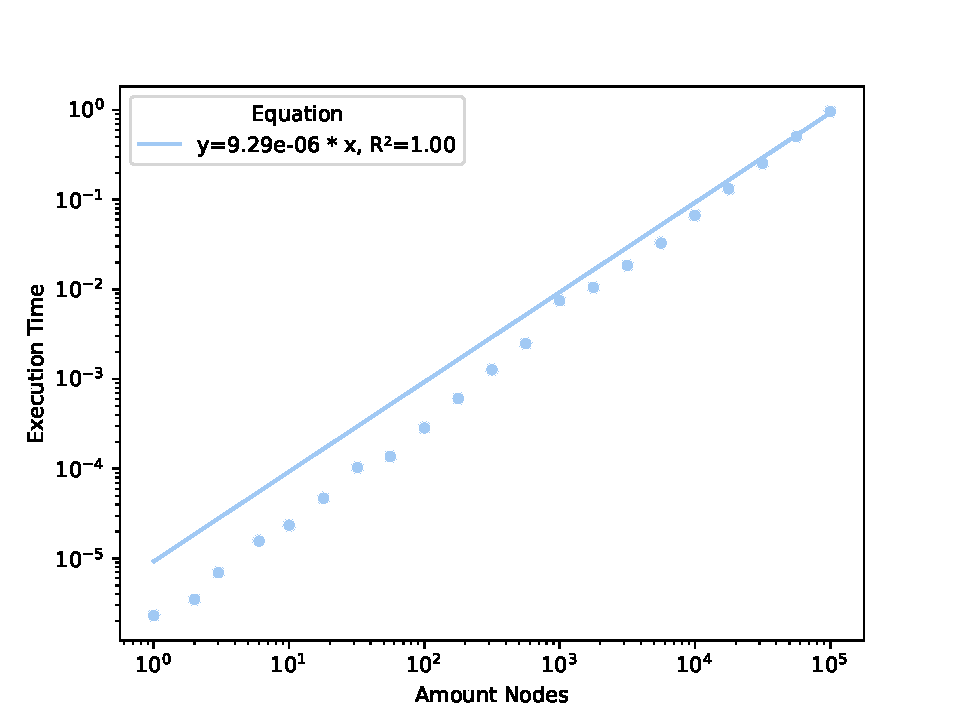
\includegraphics[width=.6\textwidth]{plots/run-2/time/benchmark_generic_cata_sum.pdf}
%     \caption{Execution time for Generic Cata Sum}
%     \label{fig-exec-time-gen-cata-sum}
% \end{figure}

% \begin{figure}[H]
%     \centering
%     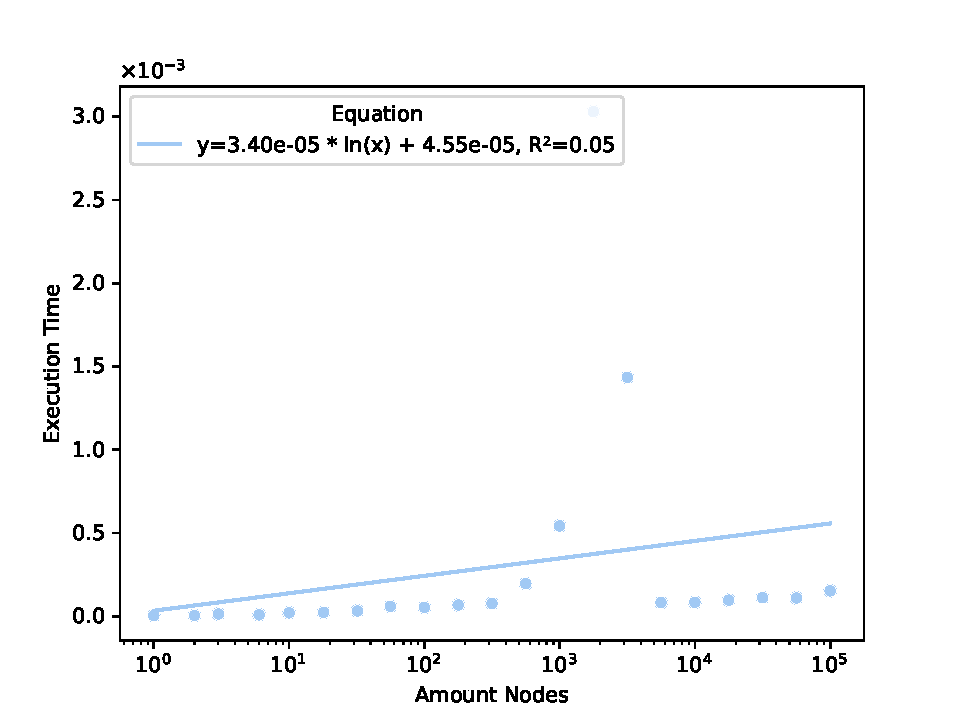
\includegraphics[width=.6\textwidth]{plots/run-2/time/benchmark_incremental_cata_sum.pdf}
%     \caption{Execution time for Incremental Cata Sum}
%     \label{fig-exec-time-inc-cata-sum}
% \end{figure}


\section{Memory Usage}
% \begin{figure}[H]
%     \centering
%     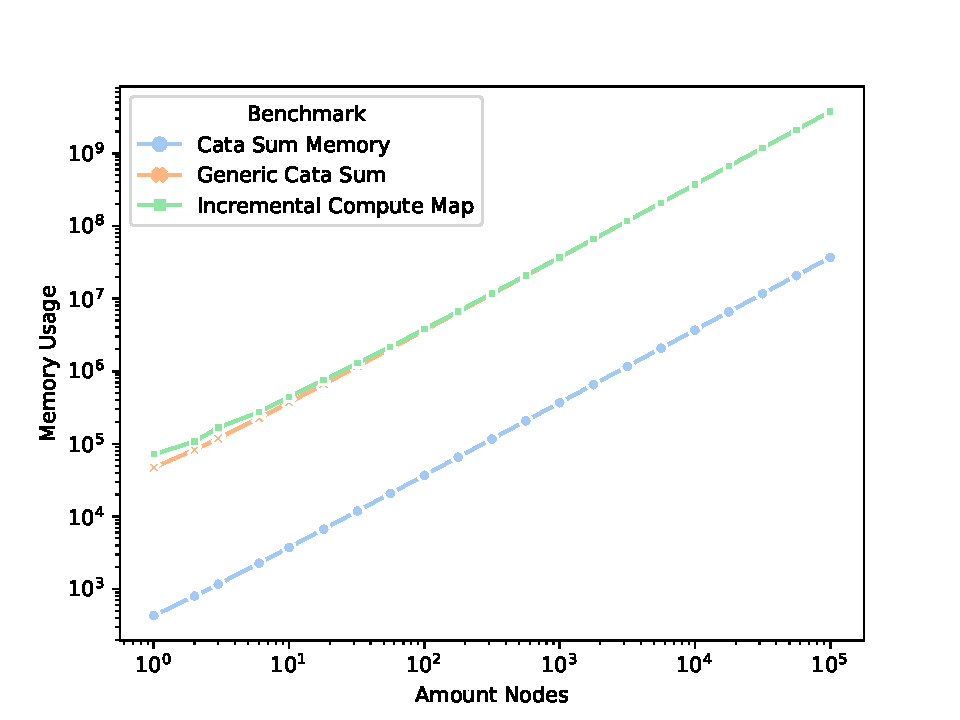
\includegraphics[width=.6\textwidth]{plots/run-2/memory/all_benchmarks.pdf}
%     \caption{Overview memory usage}
%     \label{fig-bytes-all-overview}
% \end{figure}

% \begin{figure}[H]
%     \centering
%     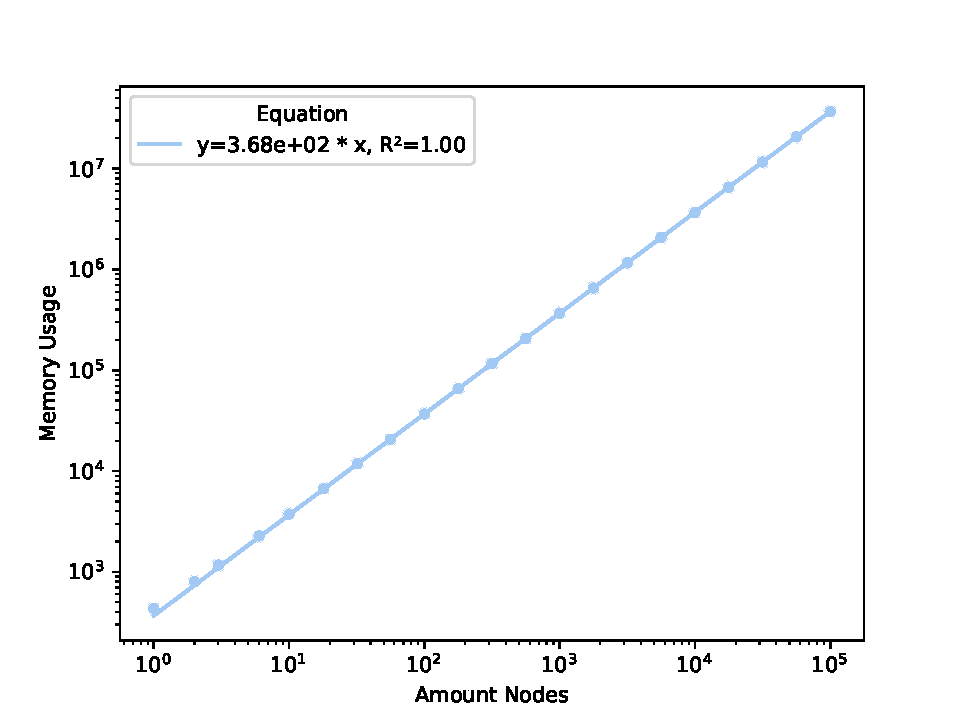
\includegraphics[width=.6\textwidth]{plots/run-2/memory/benchmark_cata_sum.pdf}
%     \caption{Memory usage for Cata Sum}
%     \label{fig-bytes-all-cata-sum}
% \end{figure}

% \begin{figure}[H]
%     \centering
%     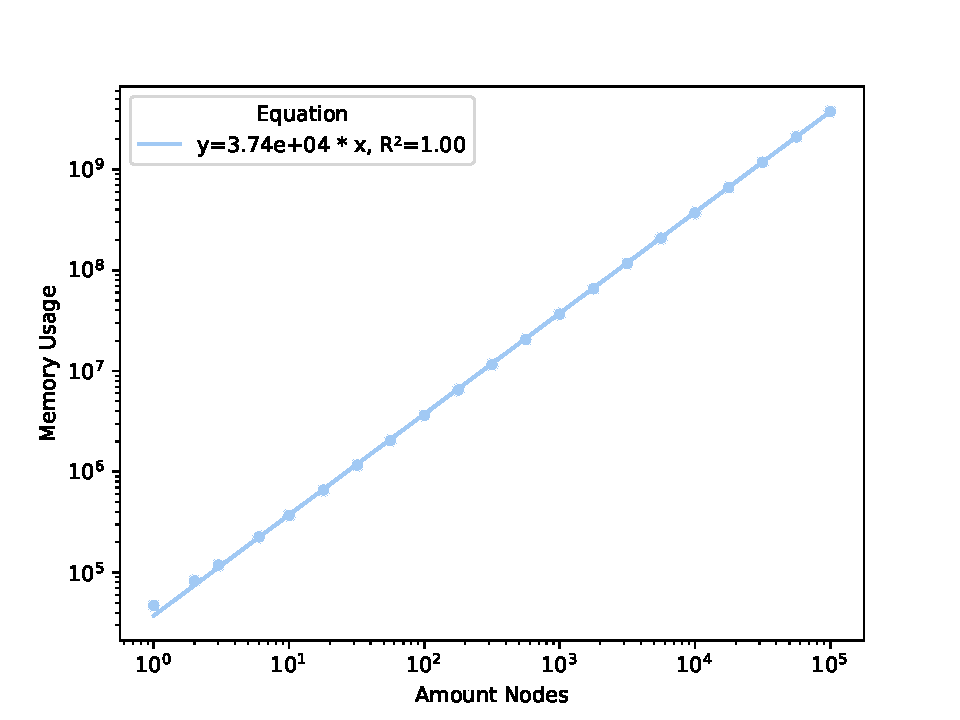
\includegraphics[width=.6\textwidth]{plots/run-2/memory/benchmark_generic_cata_sum.pdf}
%     \caption{Memory usage for Generic Cata Sum}
%     \label{fig-bytes-all-gen-cata-sum}
% \end{figure}

% \begin{figure}[H]
%     \centering
%     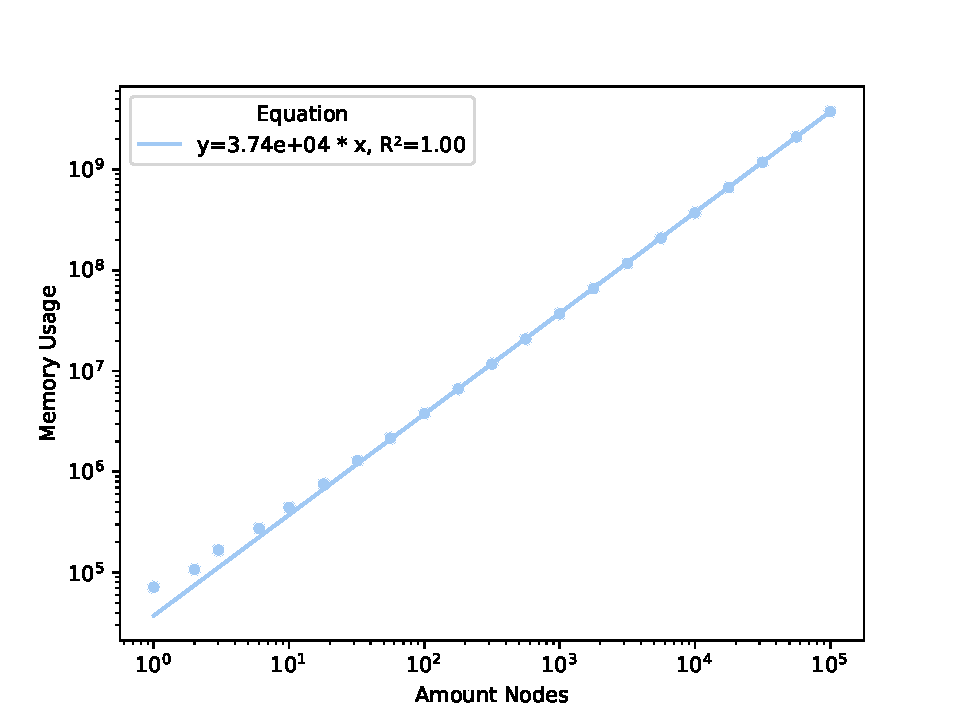
\includegraphics[width=.6\textwidth]{plots/run-2/memory/benchmark_incremental_cata_sum.pdf}
%     \caption{Memory usage for Incremental Cata Sum}
%     \label{fig-bytes-all-inc-cata-sum}
% \end{figure}

\section{Comparison Memory Strategies}
% \begin{figure}[H]
%     \centering
%     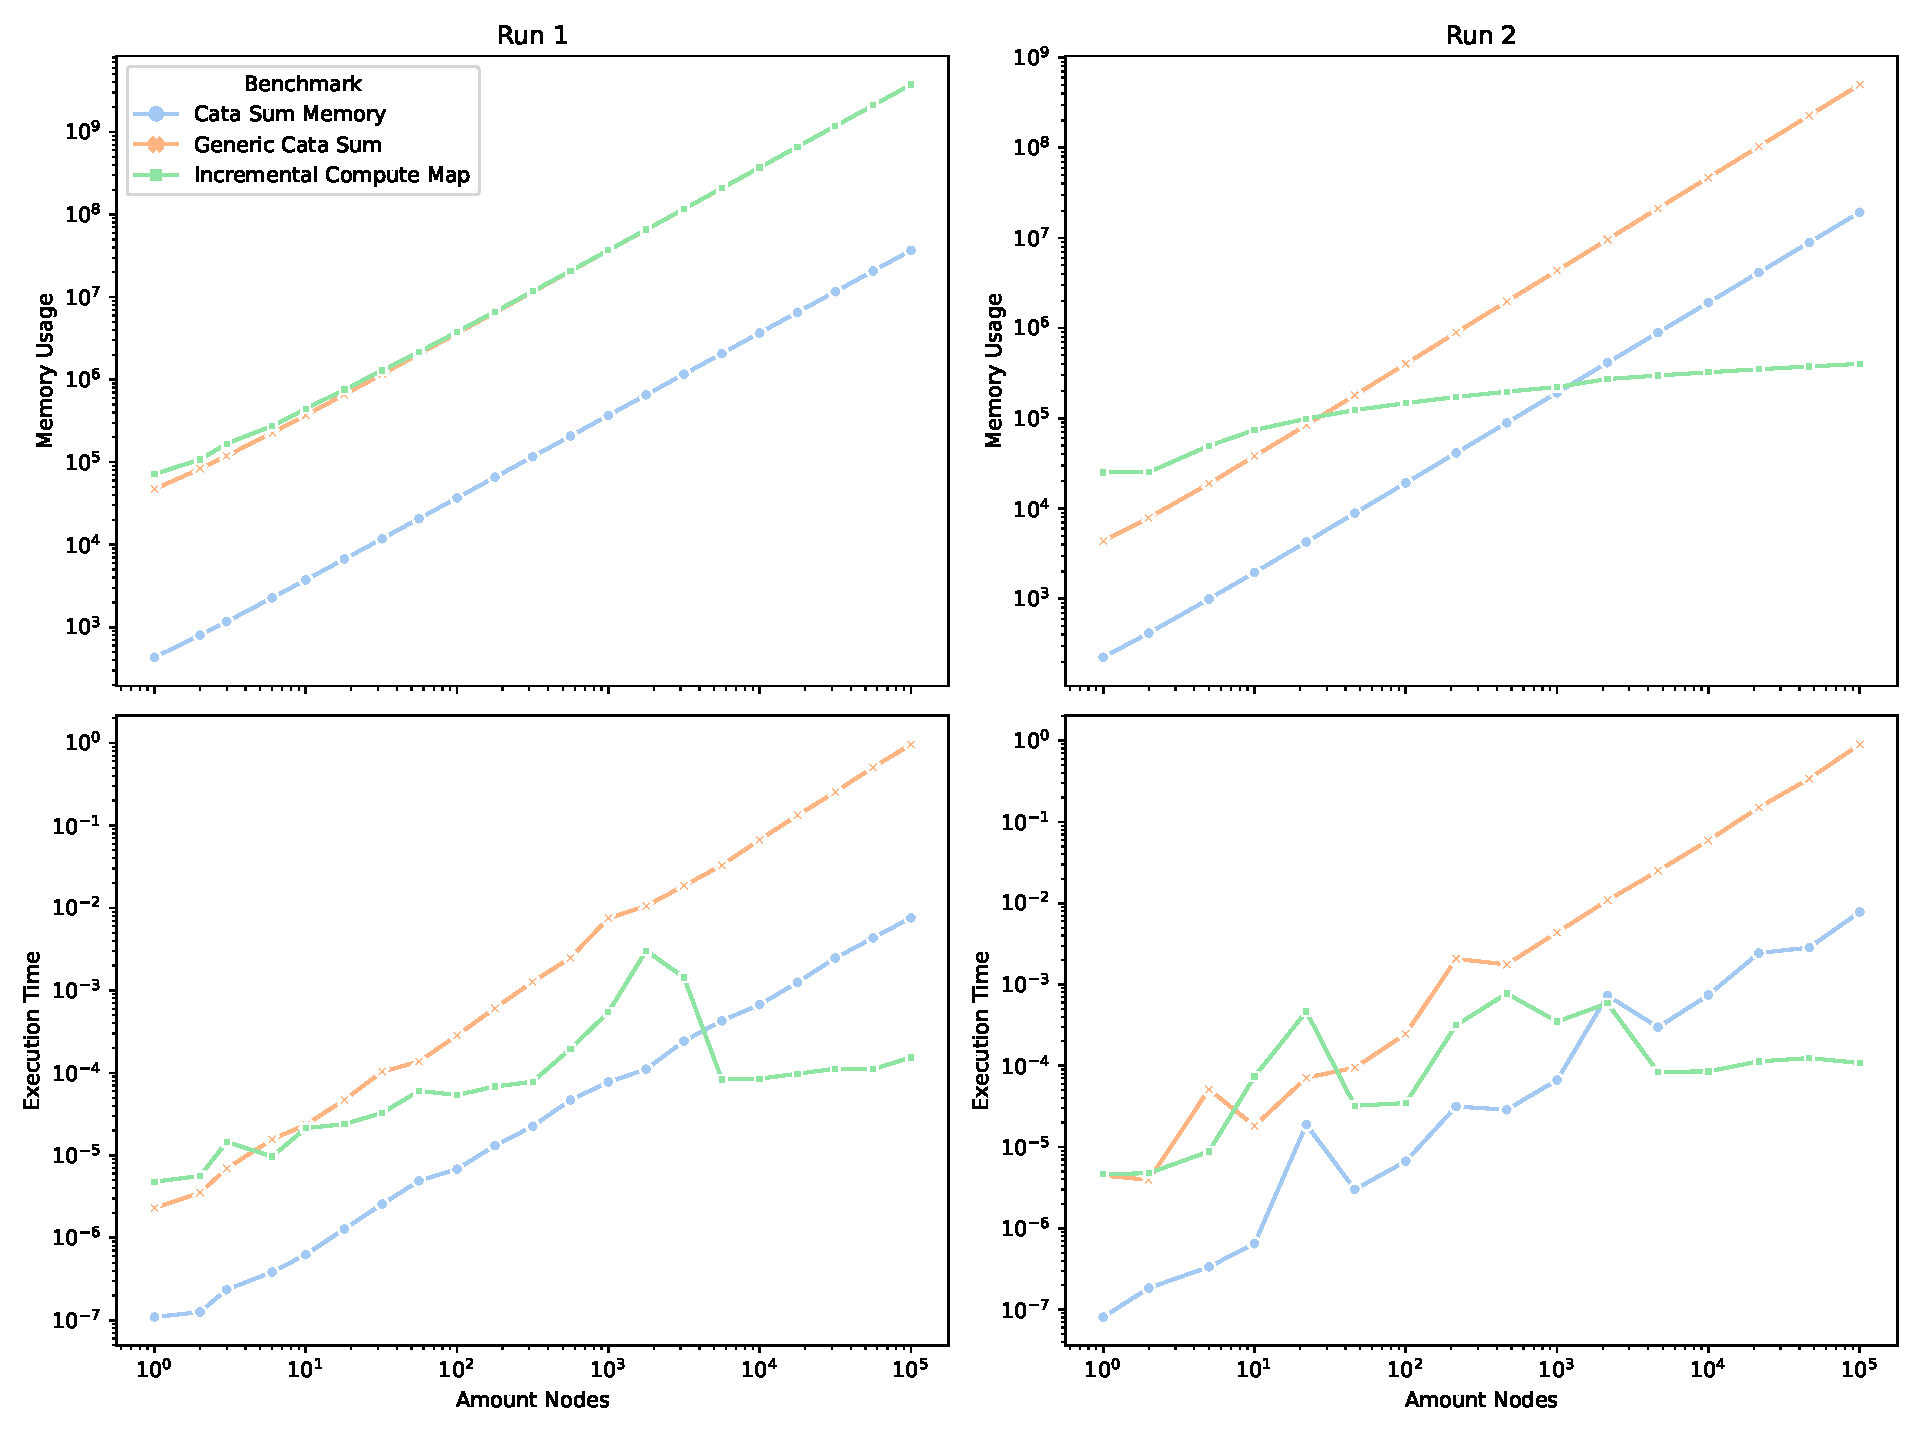
\includegraphics[width=.9\textwidth]{plots/run-2_run-1/comparison_benchmarks.pdf}
%     \caption{Comparison Memory Strategy}
%     \label{fig-comp-mem-strat}
% \end{figure}

% \newpage
% \input{sections/planning.tex}

\newpage
\section{Appendix}
\appendix

\section{Implementation Memo Cata}

\subsection{Definition Generic Datatypes}
\label{app-def-generic-datatypes}
\begin{minted}{haskell}
data U r         = U
data I r         = I r                  
data K a r       = K a                  
data (:+:) f g r = L (f r) | R (g r)
data (:*:) f g r = (f r) :*: (g r) 
data C c f r     = C (f r)

newtype Fix f = In { out :: f (Fix f) }
\end{minted}

\subsection{Implementation Hashable}
\label{app-impl-hashable}
\begin{minted}{haskell}
class Hashable f where
  hash :: f (Fix (g :*: K Digest)) -> Digest

instance Hashable U where
  hash _ = digest "U"

instance (Show a) => Hashable (K a) where
  hash (K x) = digestConcat [digest "K", digest x]

instance Hashable I where
  hash (I x) = digestConcat [digest "I", getDigest x]
    where
      getDigest :: Fix (f :*: K Digest) -> Digest
      getDigest (In (_ :*: K h)) = h

instance (Hashable f, Hashable g) => Hashable (f :+: g) where
  hash (L x) = digestConcat [digest "L", hash x]
  hash (R x) = digestConcat [digest "R", hash x]

instance (Hashable f, Hashable g) => Hashable (f :*: g) where
  hash (x :*: y) = digestConcat [digest "P", hash x, hash y]

instance (Hashable f) => Hashable (C c f) where
  hash (C x) = digestConcat [digest "C", hash x]
\end{minted}

\subsection{Implementation Merkle}
\label{app-impl-merkle}
\begin{minted}{haskell}
type Merkle f = Fix (f :*: K Digest)

merkleG :: Hashable f 
        => f (Fix (g :*: K Digest)) 
        -> (f :*: K Digest) (Fix (g :*: K Digest))
merkleG f = f :*: K (hash f)

merkle :: (Regular a, Hashable (PF a), Functor (PF a)) 
       => a -> Merkle (PF a)
merkle = In . merkleG . fmap merkle . from
\end{minted}

\subsection{Implementation Cata Merkle}
\label{app-impl-cata-merkle}
\begin{minted}{haskell}
cataMerkleState :: (Functor f, Traversable f)
                => (f a -> a) -> Fix (f :*: K Digest) 
                -> State (M.Map Digest a) a
cataMerkleState alg (In (x :*: K h)) = do m <- get
  case M.lookup h m of
    Just a -> return a
    Nothing -> do y <- mapM (cataMerkleState alg) x
                  let r = alg y
                  modify (M.insert h r) >> return r

cataMerkle :: (Functor f, Traversable f)
           => (f a -> a) -> Fix (f :*: K Digest) -> (a, M.Map Digest a)
cataMerkle alg t = runState (cataMerkleState alg t) M.empty
\end{minted}

\subsection{Implementation Zipper Merkle}
\label{app-impl-zipper-merkle}
\begin{minted}{haskell}
data Loc :: * -> * where
  Loc :: (Zipper a) => Merkle a 
                    -> [Ctx (a :*: K Digest) (Merkle a)] 
                    -> Loc (Merkle a)

modify :: (a -> a) -> Loc a -> Loc a
modify f (Loc x cs) = Loc (f x) cs

updateDigest :: Hashable a => Merkle a -> Merkle a
updateDigest (In (x :*: _)) = In (merkleG x)

updateParents :: Hashable a => Loc (Merkle a) -> Loc (Merkle a)
updateParents (Loc x []) = Loc (updateDigest x) []
updateParents (Loc x cs) = updateParents
                          $ expectJust "Exception: Cannot go up"
                          $ up (Loc (updateDigest x) cs)

updateLoc :: Hashable a => (Merkle a -> Merkle a) 
                        -> Loc (Merkle a) -> Loc (Merkle a)
updateLoc f loc = if   top loc'
                  then loc'
                  else updateParents 
                       $ expectJust "Exception: Cannot go up" (up loc')
  where
    loc' = modify f loc
\end{minted}

\section{Regular}

\subsection{Zipper}
\begin{minted}{haskell}
data instance Ctx (K a) r
data instance Ctx U r
data instance Ctx (f :+: g) r = CL (Ctx f r) | CR (Ctx g r)
data instance Ctx (f :*: g) r = C1 (Ctx f r) (g r) | C2 (f r) (Ctx g r)
data instance Ctx I r = CId
data instance Ctx (C c f) r = CC (Ctx f r)
data instance Ctx (S s f) r = CS (Ctx f r)
\end{minted}

\newpage
\printbibliography

\end{document}